\subsubsection{Übersicht}
Die Elektronik ist organisiert in einem modularen Verbund von verschiedenen
Funktionsgruppen. Nebst den elementaren Einheiten wie Motoren und zugehörigen
Treibern gehören auch etwa Pegelwandler und Sensoren dazu. Die Abbildung
\ref{fig:et-block} zeigt schematisch den Zusammenhang dieser Komponenten.


\begin{figure}[h!]
	\centering	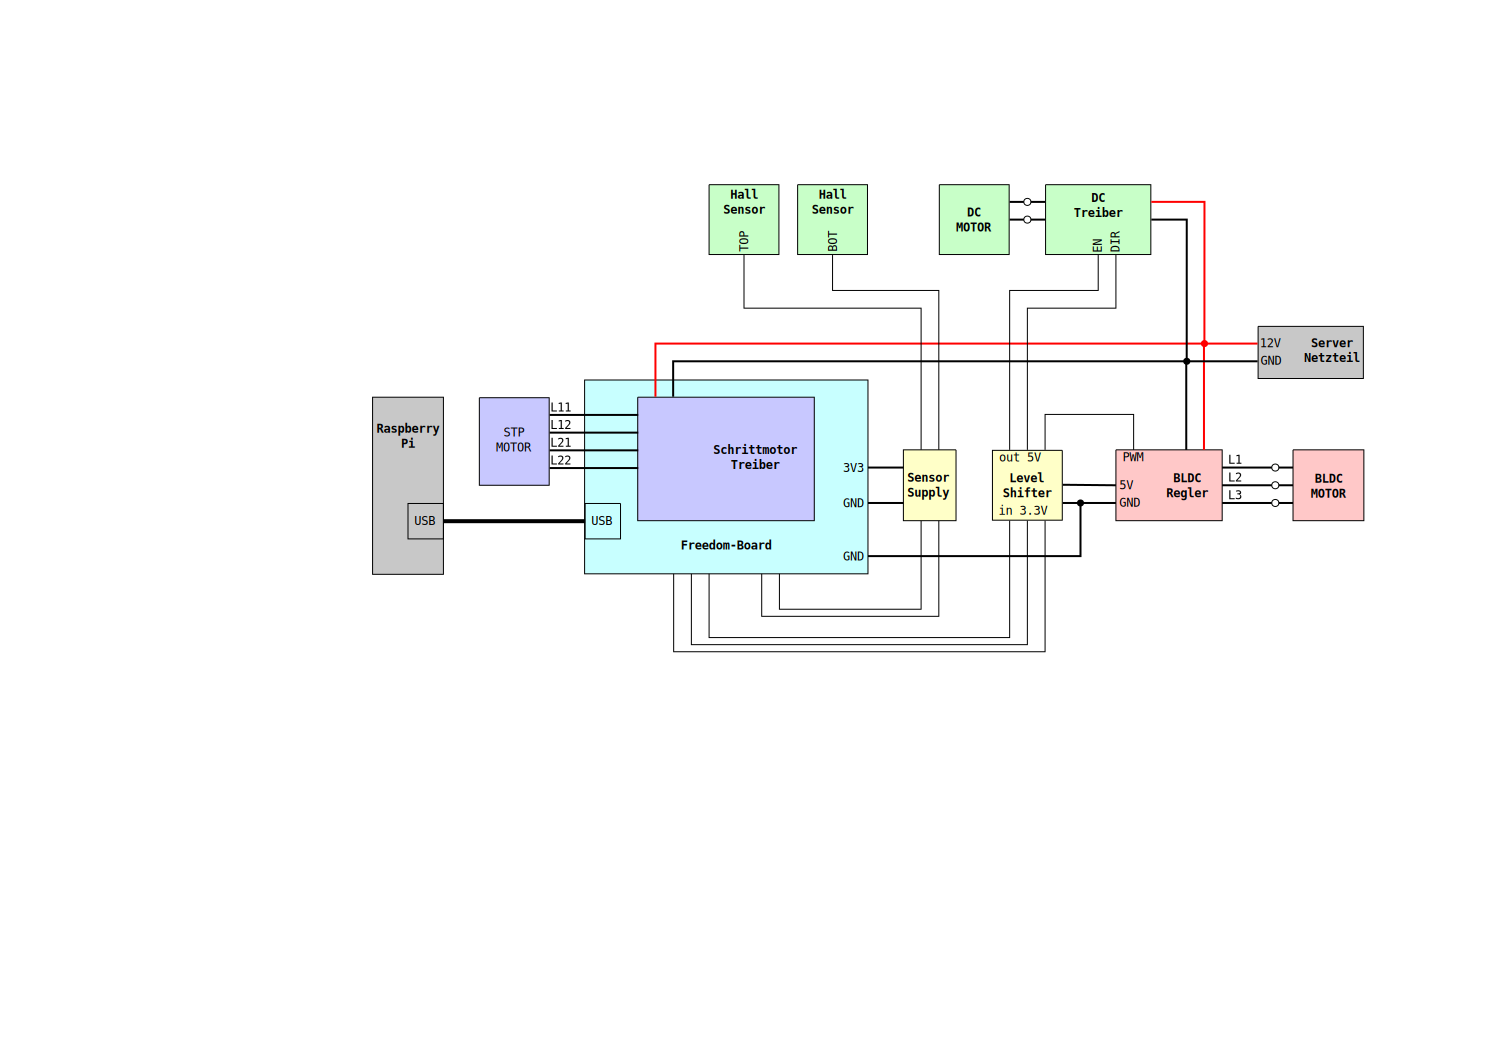
\includegraphics[width=0.95\textwidth]{../../fig/blockdiagram.pdf}
	\caption{Blockschaltbild der Elektrokomponenten}
	\label{fig:et-block}
\end{figure}
